%%% Version 3.4 Generated 2022/06/14 %%%
%%% You will need to have the following packages installed: datetime, fmtcount, etoolbox, fcprefix, which are normally inlcuded in WinEdt. %%%
%%% In http://www.ctan.org/ you can find the packages and how to install them, if necessary. %%%
%%%  NB logo1.jpg is required in the path in order to correctly compile front page header %%%

%\documentclass[utf8]{FrontiersinHarvard}

%
% PLEASE NOTE WE USE ACMART TEMPORARILY SO WE CAN SEE THE TOC
%
%\documentclass[utf8]{acmart} % for articles in journals

\documentclass[utf8]{FrontiersinVancouver} % for articles in journals

\usepackage{etoolbox} 
\newbool{SUBMISSION}
%\boolfalse{SUBMISSION}
\booltrue{SUBMISSION} 

\DeclareGraphicsExtensions{.pdf,.png,.jpg}

% \DeclareGraphicsExtensions{.jpg,.pdf,.png}


%\documentclass[utf8]{frontiersinFPHY_FAMS} % Vancouver Reference
%Style (Numbered) for articles in the journals "Frontiers in Physics"
%and "Frontiers in Applied Mathematics and Statistics"

\setcitestyle{square} % for articles in the journals "Frontiers in Physics" and "Frontiers in Applied Mathematics and Statistics" 


\usepackage{tcolorbox}
\usepackage{url}
\usepackage{lineno}
\usepackage[hidelinks]{hyperref}
\usepackage{microtype}
\usepackage{subcaption}
\usepackage[onehalfspacing]{setspace}
\usepackage{comment}
\usepackage{xcolor}
\usepackage[color=pink]{todonotes}
\usepackage{fancyvrb}
\usepackage{xcolor}
\usepackage[T1]{fontenc}
\usepackage{listings}

\lstset{
  % basicstyle=\scriptsize\ttfamily,
  basicstyle=\fontsize{10}{10}\ttfamily,
  breaklines=true,
  keywordstyle=\color{BrickRed},
  moredelim=[s][\color{BrickRed}]{\{}{\}},
  % moredelim=[s][\bfseries]{workflow:}{\n},
  % moredelim=[s][\bfseries]{nodes:}{\n},
  % literate={\{}{{\textbf{\{}}}1
  % literate={workflow:}{{{\bfseries workflow:}}}9,
  % literate={nodes:}{{{\bfseries nodes:}}}6,
  escapeinside={(*}{*)}
}

% these do not use shell escape!
% therefore they are arxiv safe

\lstdefinestyle{python}{
  language=Python,
  basicstyle=\scriptsize\ttfamily,
  keywordstyle=\color{blue},
  commentstyle=\color{green!50!black},
  stringstyle=\color{Bittersweet},
  showstringspaces=false,
  breaklines=true
}

\lstdefinestyle{sh}{
  language=sh,
  basicstyle=\scriptsize\ttfamily,
  keywordstyle=\color{blue},
  commentstyle=\color{green!50!black},
  stringstyle=\color{Bittersweet},
  showstringspaces=false,
  breaklines=true,
  keywords={singularity,echo,cms,export,cd,mkdir,nvidia-smi,python,seff}
}

\newcommand{\TODO}[2]{\todo[inline]{{\bf \color{red} #1} #2}}
\newcommand{\REPLACE}[2]{{\color{red}\it #1} \begin{quote}{\color{blue}#2}\end{quote}}
%\newcommand{\REPLACE}[2]{\begin{quote}\textcolor{red}{#1}\end{quote}\\{\textcolor{blue}{#2}}

\newcommand{\YES}{yes}

% \makeatletter\newcommand{\tableofcontents}{\@starttoc{toc}}\makeaother


\linenumbers


\def\keyFont{\fontsize{8}{11}\helveticabold }

\def\firstAuthorLast{von Laszewski {et~al.}} 
\def\Authors{Gregor von Laszewski\,$^{1,*}$,
Wesley Brewer,$^{3}$,
Andrew Shao,$^{4}$,
% J.P. Fleischer,$^{1}$
% Harshad Pitkar,,$^{5}$
Geoffrey. C. Fox,$^{1}$
}

% Affiliations should be keyed to the author's name with superscript
% numbers and be listed as follows: Laboratory, Institute, Department,
% Organization, City, State abbreviation (USA, Canada, Australia), and
% Country (without detailed address information such as city zip codes
% or street names).

% If one of the authors has a change of address, list the new address
% below the correspondence details using a superscript symbol and use
% the same symbol to indicate the author in the author list.

\def\Address{$^{1}$
Biocomplexity Institute,
University of Virginia,
% Town Center Four,
% 994 Research Park Boulevard,
 Charlottesville, VA, 22911, USA

$^{2}$
Oak Ridge National Laboratory,
P.O. Box 2008,
Oak Ridge, TN 37831, USA

$^{3}$
Hewlett Packard Enterprise,
Victoria, British Columbia, Canada

% $^{5}$
% Cummins
% Columbus, IN 47201
% City, State, USA
}


% The Corresponding Author should be marked with an asterisk Provide
% the exact contact address (this time including street name and city
% zip code) and email of the corresponding author

\def\corrAuthor{Gregor von Laszewski, Biocomplexity Institute,
University of Virginia,
Town Center Four,
994 Research Park Boulevard,
 Charlottesville, VA, 22911, USA
}

\def\corrEmail{laszewski@gmail.com}

\newcommand{\TITLE}{
Experiment Execution in Support of Community Benchmarks Workflows for HPC
}


\begin{document}

% outcomment toc when submitting

\onecolumn

\begin{comment}
%
% FOR FINAL VERSION OUTCOMMENT
%
%\clearpage

%\listoftodos
\setcounter{tocdepth}{4}
\makeatletter\newcommand{\tableofcontents}{\@starttoc{toc}}\makeaother


{\bf \TITLE}

{\Authors}

{\Address}

\bigskip

\tableofcontents

%
% OUTCOMMENT LINES ABOVE
%
\end{comment}

\title{\TITLE}



\firstpage{1}

\author[\firstAuthorLast ]{\Authors} %This field will be automatically populated
\address{} %This field will be automatically populated
\correspondance{} %This field will be automatically populated

\extraAuth{}

% If there are more than 1 corresponding author, comment this line and
%uncomment the next one.  \extraAuth{corresponding Author2
%\\ Laboratory X2, Institute X2, Department X2, Organization X2,
%Street X2, City X2 , State XX2 (only USA, Canada and Australia), Zip
%Code2, X2 Country X2, email2@uni2.edu}


\maketitle

% For Original Research Articles \citep{conference}, Clinical Trial
% Articles \citep{article}, and Technology Reports \citep{patent}, the
% introduction should be succinct, with no subheadings \citep{book}. For
% Case Reports the Introduction should include symptoms at presentation
% \citep{chapter}, physical exams and lab results \citep{dataset}.



{\bf\parindent0pt Scope statement}

{\em Not part of the main text but needs to be submitted when submitting to the journal}

{\em Provide a short statement to justify how the contents of your manuscript fit within the scope of the selected journal and specialty. Selecting the best matching journal and specialty will ensure the fastest peer review process, and prevent rejections for scope unsuitability.}


{\bf\parindent0pt Details of the solicitation}

\begin{itemize}
\item Deadline is 30 September 2024. 
    
    \item Journal/Specialty: Frontiers in High Performance Computing - section Architecture and Systems

\item Research Topic Title: Infrastructure for Workflow Systems

\item Topic Editor(s): Justin M Wozniak, Andre Merzky, Mihael Hategan-Marandiuc

\item The special issue aims to tackle the complexity of workflow systems by encouraging a bottom-up design in which necessary and well-defined components are used to assemble and construct workflow systems. 

\item We seek articles that: explore the nature and properties of such components through architectural and design constraints or through specific use cases that are generalizable
introduce new and specific workflow components, articulating their necessity for workflow systems
identify novel ways of integrating existing components into workflow systems
describe the integration of specific components into existing workflow systems
introduce models, frameworks, and tools which reduce the complexity of designing, implementing, and reasoning about workflows and workflow systems
Priority will be given to works whose applicability furthers the understanding of workflows and workflow systems.


\end{itemize}




\end{verbatim}


\newpage

\begin{abstract}

\section{}

leadership class computing add ... term and section
difference between doe and NSF .... ??? I do not even know. 
fairly large machines no matter if doe or not
order of 1000+ nodes we need to come up with some definition

university HPC vs Leadership class
tier-0 hpc agglomerated in top 500 which in top 500?

put link her of definitan.

define scale
also distingushed by examples.


hyperscale = datacenter mace 2.2 into 2.4 


\citep{cloudmesh-ee}

issue how to get urls into refernces.

development challang section



Over many decades High Performance Computing systems have been made available to the research community through research activities as well as commercially available solutions. The use of such systems has traditionally been restrictive due to the high costs of computing resources as well as the complex software to offer them efficiently to the community. Over time we saw also the utilization of federated resources such as Grids, Clouds, and todays hyperscale data centers. Still despite the many software systems and frameworks in support of these resources the utilization of them has been a challange, especially in the academic community educating the next generation of scientists. We also found that the use of benchmarks on various machines even if they are not federated play a significant hurdle in advertising a compute resource capability to the community. While popular frameworks such as Gatways and on the other spectrum Jupyter notebooks promise the simplification of the use, It is still important that scientific benchmarks are available that outline how such machines can be best utilized. This is best done in the form of workflow templates for the scientific application that can then be adapted accordingly to other scientific applications.

Within this paper, we focus first on identifying some very common usage patterns that outline which workflow templates that we have found most useful.. Naturally there are many other patterns available that may be addressed by other frameorks. However, we focus here on templates that have been common to us based on decades of use of HPC system dating back to the early parallel computers.
We especially have learned from our experience with the MLCommons Science working group that these issues are of significance and addressing them through simple tools improves the readiness of the community. Hence they can be integrated in what we term benchmark-carpentry which is one particular aspect of our workflow applications.

We have independently verified our need while developing two different libraries that upon closer inspection provide a large amount of overlap in functionality. These systems are the Experiment Executor which is part of a larger bag of services distributed as part of cloudmesh that has been used for more than a decade, as well as SmartSim developed by Hewlett Packard which similarly addresses experiment management. The application has been tested on various scientific applications. In our earlier work, this was done on cloudmask and earthquake prediction. Here we focus on the need to develop a surrogate for computational fluid dynamics.


\tiny \keyFont{ \section{Keywords:} deep learning, benchmarking, hyper
  parameter search, hybrid heterogeneous hyperparameter search,
  scientific benchmark, cloudmesh, SmartSim}

% All article types: you may provide up to 8 keywords; at least 5 are mandatory.

\end{abstract}



%%%%%%%%%%%%%%%%%%%%%%%%%%%%%%%%%%%%%%%%%%%%%%%%%%%%%%%%%%%%%%%%%%%%%%%%%%%%%%%
\section{Introduction}
%%%%%%%%%%%%%%%%%%%%%%%%%%%%%%%%%%%%%%%%%%%%%%%%%%%%%%%%%%%%%%%%%%%%%%%%%%%%%%%

%%%%%%%%%%%%%%%%%%%%%%%%%%%%%%%%%%%%%%%%%%%%%%%%%%%%%%%%%%%%%%%%%%%%%%%%%%%%%%%
\subsection{HPC Benchmarks}
%%%%%%%%%%%%%%%%%%%%%%%%%%%%%%%%%%%%%%%%%%%%%%%%%%%%%%%%%%%%%%%%%%%%%%%%%%%%%%%

CPU
GPU
Data storage
Energy

Compute time
Wait time

Partition properties

Top 500

``The Top500 list the 500 fastest computer system being used today. In 1993 the collection was started and has been updated every 6 months since then. The report lists the sites that have the 500 most powerful computer systems installed. The best Linpack benchmark performance achieved is used as a performance measure in ranking the computers. The TOP500 list has been updated twice a year since June 1993.'' \citep{www-top500}

HPCG 

``The TOP500 list has incorporated the High-Performance Conjugate Gradient (HPCG) benchmark results, which provide an alternative metric for assessing supercomputer performance. This score is meant to complement the HPL measurement to give a fuller understanding of the machine.''  \citep{www-top500}

Green 500

Energy Efficiency (GFlops/watts) \citep{green500}

Application oriented benchmarks based on discipline

MLCommons Benchmark for machine learning


\section{HPC Benchmark  Workflows}

install software
reserve machine to exclusive use
prepare batch jobs for the run
evaluate and validate the performance
compare results
submit results




%%%%%%%%%%%%%%%%%%%%%%%%%%%%%%%%%%%%%%%%%%%%%%%%%%%%%%%%%%%%%%%%%%%%%%%%%%%%%%%
\subsection{Benchmark Carpentry for Experiment Execution}
%%%%%%%%%%%%%%%%%%%%%%%%%%%%%%%%%%%%%%%%%%%%%%%%%%%%%%%%%%%%%%%%%%%%%%%%%%%%%%%

FAIR

result templates


%%%%%%%%%%%%%%%%%%%%%%%%%%%%%%%%%%%%%%%%%%%%%%%%%%%%%%%%%%%%%%%%%%%%%%%%%%%%%%%
\section{Experiment Execution Templates}
%%%%%%%%%%%%%%%%%%%%%%%%%%%%%%%%%%%%%%%%%%%%%%%%%%%%%%%%%%%%%%%%%%%%%%%%%%%%%%%

%%%%%%%%%%%%%%%%%%%%%%%%%%%%%%%%%%%%%%%%%%%%%%%%%%%%%%%%%%%%%%%%%%%%%%%%%%%%%%%
\subsection{Experiment Execution on High Performance Computers}
%%%%%%%%%%%%%%%%%%%%%%%%%%%%%%%%%%%%%%%%%%%%%%%%%%%%%%%%%%%%%%%%%%%%%%%%%%%%%%%

%%%%%%%%%%%%%%%%%%%%%%%%%%%%%%%%%%%%%%%%%%%%%%%%%%%%%%%%%%%%%%%%%%%%%%%%%%%%%%%
\subsection{Experiment Execution on Hyperscale Ressource}
%%%%%%%%%%%%%%%%%%%%%%%%%%%%%%%%%%%%%%%%%%%%%%%%%%%%%%%%%%%%%%%%%%%%%%%%%%%%%%%


%%%%%%%%%%%%%%%%%%%%%%%%%%%%%%%%%%%%%%%%%%%%%%%%%%%%%%%%%%%%%%%%%%%%%%%%%%%%%%%
\subsection{Federated Experiment Execution}
%%%%%%%%%%%%%%%%%%%%%%%%%%%%%%%%%%%%%%%%%%%%%%%%%%%%%%%%%%%%%%%%%%%%%%%%%%%%%%%

From Grids back to client-side control

%%%%%%%%%%%%%%%%%%%%%%%%%%%%%%%%%%%%%%%%%%%%%%%%%%%%%%%%%%%%%%%%%%%%%%%%%%%%%%%
\subsection{Experiment Execution on Clouds}
%%%%%%%%%%%%%%%%%%%%%%%%%%%%%%%%%%%%%%%%%%%%%%%%%%%%%%%%%%%%%%%%%%%%%%%%%%%%%%%

The CoGKits for Java and Python were the predecessor to cloudmesh. While those tools focused on Grid computing interfaces for the various Grid toolkits. Cloudmesh provided the opportunity to shift its focus to services offered by cloud computing including Azure, AWS, Google, OpenStack clouds, and Chamelon Cloud via OpenStack. Here cloudmesh focused on the creation of a very simple mechanism to start compute resources uniformly on the various clouds while providing templates that offer similar capabilities across them. As such workflows could be created that allowed switching easily be tween virtual machines. This is achieved by the cloudmesh command line and command shell that prior to any other tool allowed integrating and switching between clouds easily. Thus to start a vm on AWS, then one on Azure one could simply say

\begin{berbatim}
cms set cloud=aws
cms vm start
cms set cloud=azures
cms vm start
cms vm start --cloud=google
\end{enumerate}

cloudmesh was the first tool that promoted a setup of cloud credentials in yaml files that were used to start "templated" virtual machines with default parameters provided by these templates. Only later were similar capabilities integrated in for example,  OpenStack. Thus we can support cloud-based workflows

\begin{itemize}
    \item on one or multiple clouds
    \item cloud agnostic workflows
    \item adding easily new clouds into the workflows by integrating access points
    \item allow the integration of new clouds and their vm access protocols
\end{itemize}

As clouds have recently also integrated containers and server less computing we have prototyped the ability to stand up Kubernetes clusters (in AWS for example). As setting up such clusters is a task that is beyond the capabilities of scientists we prototyped an easy way to set them up including default security and network capabilities. The integration into cloudmesh is conducted through the cloudmesh plugin mechanism that ads dynamically this capability with a simple pip install.

Most recently a shift in scientific computing has taken place that emphasizes the use of GPU compute resources. For this reason AWS has added the ability to bootstrap in the cloud parallel clusters including their control through SLURM. Obviously, this could also be leveraged by a scientist that may not have a super computer at their facility or wants to conduct an HPC workload in the cloud. However the configuration and setup is something most scientists do not want to be bothered with. Their goal is the access to the compute resources. Our cloud cluster plugin to cloudmesh therefor contains the ability to deploy a cloud cluster with or without GPUs, as well as the size of the working node with the help of a single command to which we specify such things as the name of the cluster, how many nodes, and if and which GPUs should be used. Obviously that can all be configured through AWS cloud formation, however, the setup and the configuration parameters are too complex to just support this general workflow case. Hence we have provided a simplified YAML configuration file that can also be specified on the command line  and allows reasonable flexibility. One such flexibility is to define multiple clusters that may be busy working on multiple things. It is to be noted that the setup of such cluster costs a significant time (such as 15 minutes) but this is time in contrast to the expected runtimes conducted on such clusters. It also provides a meaningful estimation on when such clusters may be used. For sure, they should not be used by a single user with only a few seconds compute time.  The experiment executions as part of the scientific discover workflow should be much larger.





%%%%%%%%%%%%%%%%%%%%%%%%%%%%%%%%%%%%%%%%%%%%%%%%%%%%%%%%%%%%%%%%%%%%%%%%%%%%%%%
\section{Experiment Executors}
%%%%%%%%%%%%%%%%%%%%%%%%%%%%%%%%%%%%%%%%%%%%%%%%%%%%%%%%%%%%%%%%%%%%%%%%%%%%%%%

%%%%%%%%%%%%%%%%%%%%%%%%%%%%%%%%%%%%%%%%%%%%%%%%%%%%%%%%%%%%%%%%%%%%%%%%%%%%%%%
\subsection{Experiment Executor (Cloudmesh Plugin)}
%%%%%%%%%%%%%%%%%%%%%%%%%%%%%%%%%%%%%%%%%%%%%%%%%%%%%%%%%%%%%%%%%%%%%%%%%%%%%%%

%%%%%%%%%%%%%%%%%%%%%%%%%%%%%%%%%%%%%%%%%%%%%%%%%%%%%%%%%%%%%%%%%%%%%%%%%%%%%%%
\subsection{SmartSim}
%%%%%%%%%%%%%%%%%%%%%%%%%%%%%%%%%%%%%%%%%%%%%%%%%%%%%%%%%%%%%%%%%%%%%%%%%%%%%%%
SmartSim is a Python-based, open-source library that allows users to describe
and execute hybrid AI/ModSim workflows using an in-memory datastore to exchange
information. It has been used in a variety of computational fluid dynamics
applications where AI techniques (1) embedded within the numerical solver for
turbulence parameterizations and as an interpolator for moving meshes and (2)
applied outside the simulation to create reinforcement learning and automatic
parameter estimation applications.



Inferencing capability is accomplished through Redis, key-value database, and
the RedisAI module. SmartRedis is a lightweight library (and a sibling to
SmartSim) that simulation developers can embed in their C, C++, and Fortran
codebases. The Redis database can be sharded across multiple nodes, each one
capable of performing inference. Notably requests from multiple clients can be
batched together, minimizing penalties associated with moving small amounts of
data to/from the GPU.

Implementing the OSMI benchmark with SmartSim requires two steps. One, we wrote
a ``driver'' script that describes both the database and the application that
will request the inference. To ensure parity with Cloudmesh, the same YAML file
is ingested into the configuration of these objects. 



%%%%%%%%%%%%%%%%%%%%%%%%%%%%%%%%%%%%%%%%%%%%%%%%%%%%%%%%%%%%%%%%%%%%%%%%%%%%%%%
\section{Evaluation}
%%%%%%%%%%%%%%%%%%%%%%%%%%%%%%%%%%%%%%%%%%%%%%%%%%%%%%%%%%%%%%%%%%%%%%%%%%%%%%%

%%%%%%%%%%%%%%%%%%%%%%%%%%%%%%%%%%%%%%%%%%%%%%%%%%%%%%%%%%%%%%%%%%%%%%%%%%%%%%%
\subsection{Applications}
%%%%%%%%%%%%%%%%%%%%%%%%%%%%%%%%%%%%%%%%%%%%%%%%%%%%%%%%%%%%%%%%%%%%%%%%%%%%%%%


%%%%%%%%%%%%%%%%%%%%%%%%%%%%%%%%%%%%%%%%%%%%%%%%%%%%%%%%%%%%%%%%%%%%%%%%%%%%%%%
\subsubsection{OSMI}
%%%%%%%%%%%%%%%%%%%%%%%%%%%%%%%%%%%%%%%%%%%%%%%%%%%%%%%%%%%%%%%%%%%%%%%%%%%%%%%

Most AI workflows on HPC can be categorized in six different execution motifs: Steering, Multistage Pipeline, Inverse Design, Digital Replica, Distributed Models, and Adaptive Training \cite{brewer2024ai}. One component that shows up across multiple motifs is machine-learned surrogate models. Such models typically are used in hybrid ModSim / AI workflows, where traditional simulations are used for a large part of the workflow, and then particular aspects of the simulation, such as a turbulence or radiation model, are replaced by digital surrogates, e.g., \cite{partee2022using, martinez2022roam, bhushan2023assessment}. Because of the challenges of integrating the simulations with the AI model in a highly scalable manner, developing a benchmark was necessary to assess the performance of various configurations. Initial developments of a surrogate model benchmark, called ``smiBench'', were studied by Brewer et al. \cite{brewer2021production}. The studies showed that using a separate load balancer on each compute node, which round-robins the inference requests across multiple GPUs on the node, and also using the maximum batch size that the GPU memory allows yields optimal inference performance. This study was followed by a secondary investigation by Boyer et al. \cite{boyer2022scalable}, which investigated performance implications of the full coupling between the surrogate inference and the simulation code, and showed that using a concurrency level of two batch inference requests was optimal. 

The Open Surrogate Model Inference (OSMI) benchmark was developed as an open-source community benchmark founded upon these principles. The architecture of OSMI is shown in Fig. \ref{fig:osmi}. The benchmark supports either TensorFlow or SmartSim/PyTorch based frameworks as shown in Table \ref{tab:osmi}. Inference requests are initiated from within the simulation using a client API call (e.g., SmartRedis or gRPC API), the requests are then sent to a load balancer (e.g., HAProxy), which distributes the requests in a round-robin fashion to multiple inference servers, each bound to a single GPU. Benchmark timings are able to be measured at multiple places in the architecture, but the primary measurement of interest is how long it takes from the time an inference request is initiated from the simulation, until the response is returned back to it. As opposed to chip-level benchmarks such as MLPerf \cite{reddi2020mlperf}, OSMI is able the measure system-level performance, which includes the performance of the CPU, GPU, network, and interconnect (IC), giving a holistic performance representation of the system. This same approach was used to benchmark a wide range of HPC systems, revealing significant performance differences between seemingly similar machines, often due to factors such as different interconnect performance \cite{brewer2020inference}.

\begin{figure}[t]
    \centering
    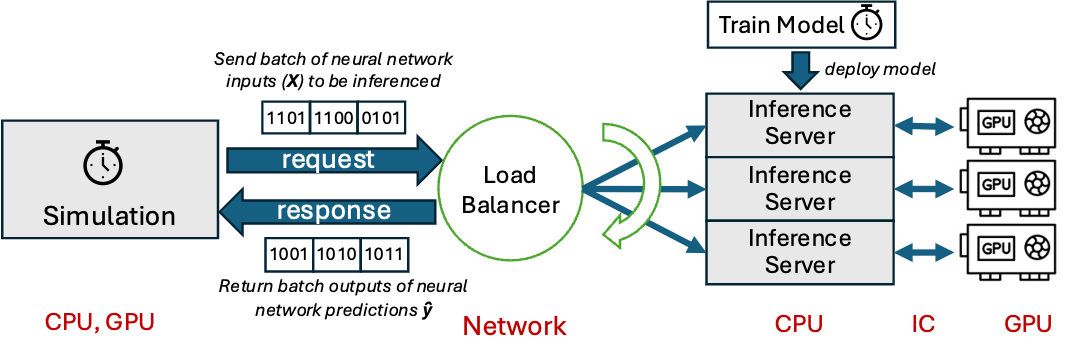
\includegraphics[width=\linewidth]{images/osmi_arch.png}
    \caption{Architecture of OSMI benchmark.}
    \label{fig:osmi}
\end{figure}

\begin{table}[t]
\centering
\renewcommand{\arraystretch}{1.5}
\begin{tabular}{llll}
\hline
\textbf{AI framework} & \textbf{Inference server} & \textbf{Client API} & \textbf{Protocol} \\ \hline
TensorFlow & TF Serving  & TF Serving API  & gRPC  \\
PyTorch    & RedisAI     & SmartRedis      & RESP  \\ \hline
\end{tabular}
\caption{OSMI-supported AI frameworks.}
\label{tab:osmi}
\end{table}

%%%%%%%%%%%%%%%%%%%%%%%%%%%%%%%%%%%%%%%%%%%%%%%%%%%%%%%%%%%%%%%%%%%%%%%%%%%%%%%
\subsubsection{Cyclic Execution }
%%%%%%%%%%%%%%%%%%%%%%%%%%%%%%%%%%%%%%%%%%%%%%%%%%%%%%%%%%%%%%%%%%%%%%%%%%%%%%%
- Reinforcement learning
- Parameter optimization
- Online training

%%%%%%%%%%%%%%%%%%%%%%%%%%%%%%%%%%%%%%%%%%%%%%%%%%%%%%%%%%%%%%%%%%%%%%%%%%%%%%
\subsection{Community Experience}
%%%%%%%%%%%%%%%%%%%%%%%%%%%%%%%%%%%%%%%%%%%%%%%%%%%%%%%%%%%%%%%%%%%%%%%%%%%%%%%

%%%%%%%%%%%%%%%%%%%%%%%%%%%%%%%%%%%%%%%%%%%%%%%%%%%%%%%%%%%%%%%%%%%%%%%%%%%%%%%
\section{Related Activities}
%%%%%%%%%%%%%%%%%%%%%%%%%%%%%%%%%%%%%%%%%%%%%%%%%%%%%%%%%%%%%%%%%%%%%%%%%%%%%%%


%%%%%%%%%%%%%%%%%%%%%%%%%%%%%%%%%%%%%%%%%%%%%%%%%%%%%%%%%%%%%%%%%%%%%%%%%%%%%%%
\section{Future Work}
%%%%%%%%%%%%%%%%%%%%%%%%%%%%%%%%%%%%%%%%%%%%%%%%%%%%%%%%%%%%%%%%%%%%%%%%%%%%%%%


%%%%%%%%%%%%%%%%%%%%%%%%%%%%%%%%%%%%%%%%%%%%%%%%%%%%%%%%%%%%%%%%%%%%%%%%%%%%%%%
\section{Conclusion}
%%%%%%%%%%%%%%%%%%%%%%%%%%%%%%%%%%%%%%%%%%%%%%%%%%%%%%%%%%%%%%%%%%%%%%%%%%%%%%%



%%%%%%%%%%%%%%%%%%%%%%%%%%%%%%%%%%%%%%%%%%%%%%%%%%%%%%%%%%%%%%%%%%%%%%%%%%%%%%%
\clearpage

\section{Nomenclature}

\subsection{Resource Identification Initiative}

{\bf Organization:} \verb|RRID:SCR_011743|

\section*{Conflict of Interest Statement}

The authors declare that the research was conducted in the absence of any commercial or financial relationships that could be construed as a potential conflict of interest.

\section*{Author Contributions}

{\em GvL} is the author of the Experiment Executor and many other components that are distributed at bag of plugins to cloudmesh.  He has modified modifications to how the OSMI benchmark operates while leveraging some of the elementary features contained in the cloudmesh experiment management. He has decades worth of HPC dating back to 1984. 

{\em GCF} is the author of the earthquake code and facilitates the interactions with the MLCommons Science Working group as a group leader of that effort. 


{\em WB} is the author of the OSMI code and benchmark. His experience from using DOE machines is integrated into this paper. {AS} is the author of SmartSim and his experience from supporting the many customers in HPE is integrated into this paper.

\section*{Funding}

Work was in part funded by the NSF CyberTraining: CIC: CyberTraining for Students and Technologies from Generation Z with the award numbers 1829704 and 2200409 and NIST 60NANB21D151T.  The work was also funded by the Department of Energy under the grant Award No. DE-SC0023452. The work was conducted at the Biocomplexity Institute and Initiative at the University of Virginia.

\section*{Acknowledgments}

We like to thank Jaques P. Fleisher for his contribution to the cloudmesh-vpn plugin for integrating split VPN as well as his independent testing of the workflow code for multiple scientific applications such as earthquake and cloudmask.

This research was sponsored in part by and used resources of the Oak Ridge Leadership Computing Facility (OLCF), which is a DOE Office of Science User Facility at the Oak Ridge National Laboratory (ORNL) supported by the U.S. Department of Energy under Contract No. DE-AC05-00OR22725.

\section*{Data Availability Statement}

The code is all in the public domain and available on GitHub at the following locations

\begin{itemize}

\item {\bf cloudmesh-cc} -- Is a code to control workflows to be executed on
  remote computing
  resources. \url{https://github.com/cloudmesh/cloudmesh-cc}

\item {\bf cloudmesh-ee} -- Is a code to generate batch scripts for
  hyperparameter studies high-performance computers so they can be
  executed on different supercomputers by multiple
  accounts. \url{https://github.com/cloudmesh/cloudmesh-ee}


\item {\bf cloudmesh-vpn} -- Is a plugin that allows to use a VPN client as part of the client focused workflow supported by the cloudmesh command and shell. Recently we added support for split VPN allowing the access to multiple resources controlled by multiple VPNs.
\url{https://github.com/cloudmesh/cloudmesh-vpn}

\item {\bf cloudmesh} -- Cloudmesh is a large collection of repositories for
  accessing cloud and HPC
  resources. \url{https://github.com/orgs/cloudmesh/repositories}

\item {\bf OSMI} -- Is a surrogate-model inference benchmark. \url{https://github.com/laszewsk/osmi-bench-new}

%\item {\bf MLCommons earthquake production code} -- The MLCommons Science
%  Working group is described at
%  \url{https://mlcommons.org/en/groups/research-science/}. This page
%  contains the links to the production-level earthquake code.

%\item {\bf MLCommons earthquake development code} -- The development version of
%  the code is available in this repository. It also contains many of
%  the analysis scripts that are not part of the production code
%  hosted by MLCommons \url{https://github.com/laszewsk/mlcommons}.

\end{itemize}


% \bibliographystyle{Frontiers-Harvard}

\bibliographystyle{Frontiers-Vancouver} % Many Frontiers journals
% use the numbered referencing system, to find the style and resources
% for the journal you are submitting to:
% https://zendesk.frontiersin.org/hc/en-us/articles/360017860337-Frontiers-Reference-Styles-by-Journal

\bibliography{vonLaszewski-frontiers-citations}





\end{document}
